\section{Auswertung}
\subsection{Dioden}
\begin{enumerate}[label=\alph*)]
	\item Stellen Sie die Kennlinien im linearen Maßstab dar, benutzen Sie dazu die korrigierten Messwerte (Spannungsfehlerschaltung beachten, Durchlassrichtung und Sperrrichtung unterschiedliche Maßstäbe, ggf. je zwei Diagramme).
	      \begin{figure}[h!]
		      \begin{center}
			      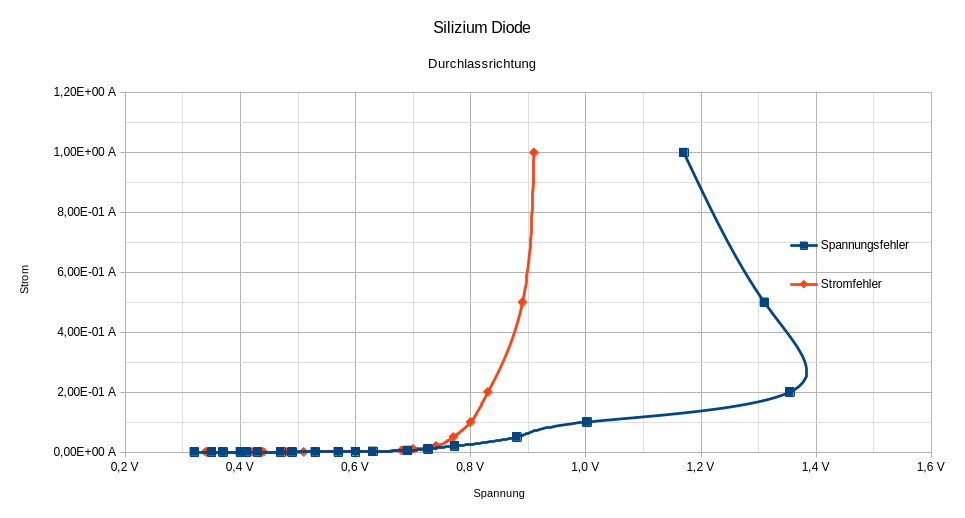
\includegraphics[width=0.85\textwidth]{img/4.1.a.1}
			      \caption{Silizium Diode in Durchlassrichtung}
		      \end{center}
	      \end{figure}

	      \begin{figure}[h!]
		      \begin{center}
			      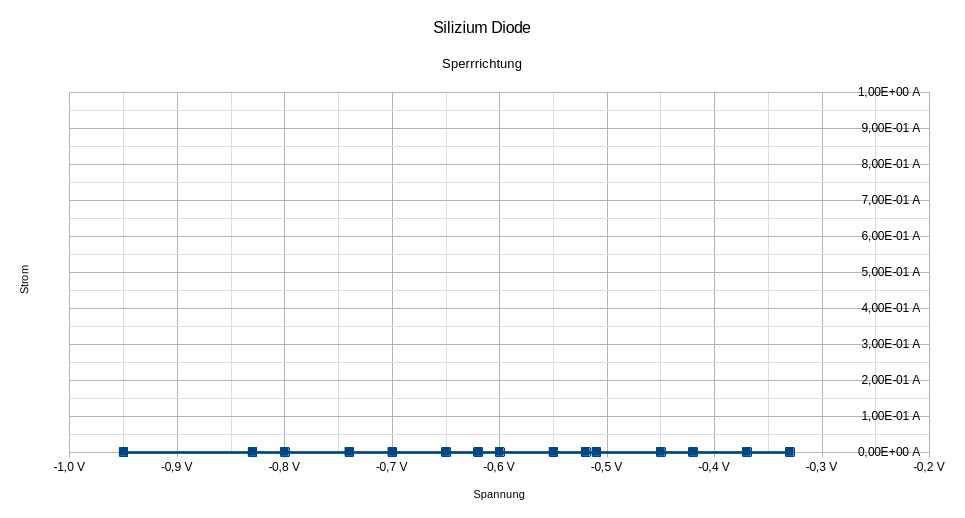
\includegraphics[width=0.85\textwidth]{img/4.1.a.2}
			      \caption{Silizium Diode in Sperrrichtung}
		      \end{center}
	      \end{figure}

	      \pagebreak

	      \begin{figure}[h!]
		      \begin{center}
			      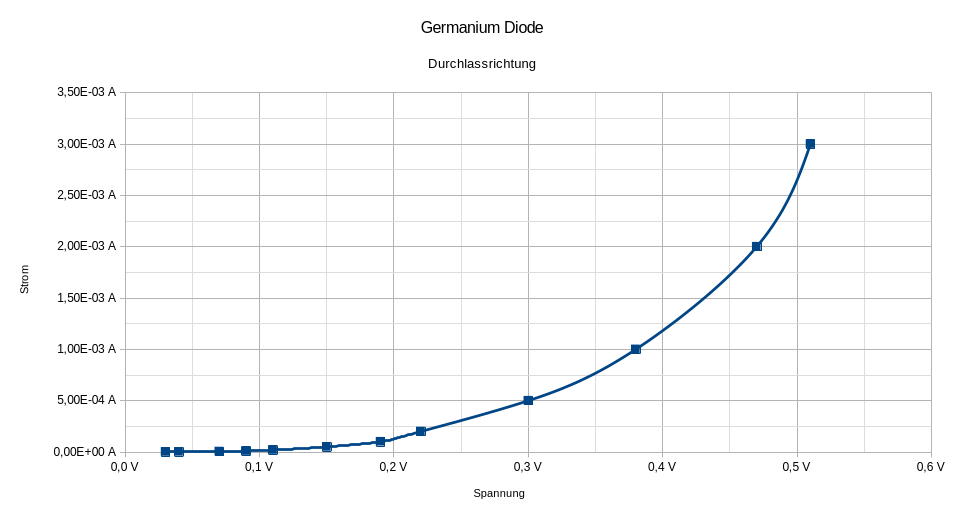
\includegraphics[width=0.85\textwidth]{img/4.1.a.3}
			      \caption{Germanium Diode in Durchlassrichtung}
		      \end{center}
	      \end{figure}

	      \begin{figure}[h!]
		      \begin{center}
			      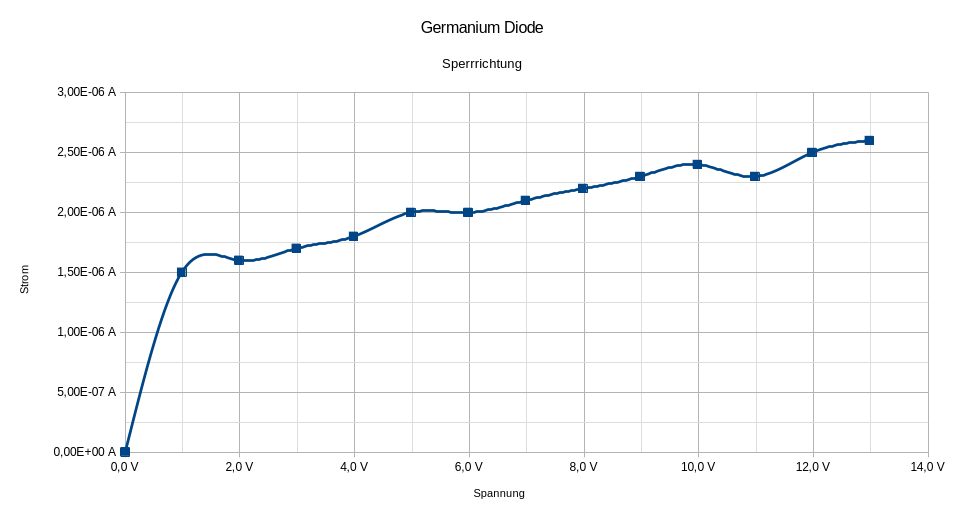
\includegraphics[width=0.85\textwidth]{img/4.1.a.4}
			      \caption{Germanium Diode in Sperrrichtung}
		      \end{center}
	      \end{figure}

	      \pagebreak

	      \begin{figure}[h!]
		      \begin{center}
			      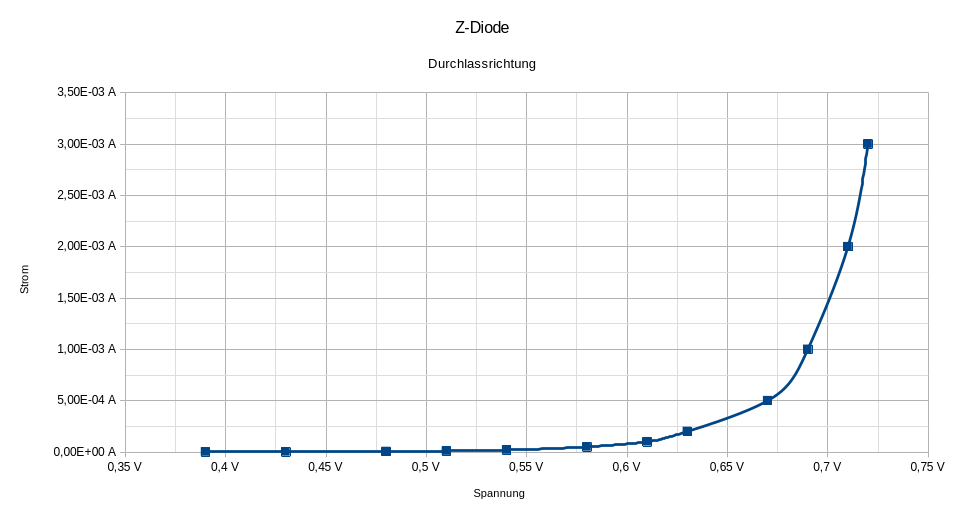
\includegraphics[width=0.85\textwidth]{img/4.1.a.5}
			      \caption{Z-Diode in Durchlassrichtung}
		      \end{center}
	      \end{figure}

	      \begin{figure}[h!]
		      \begin{center}
			      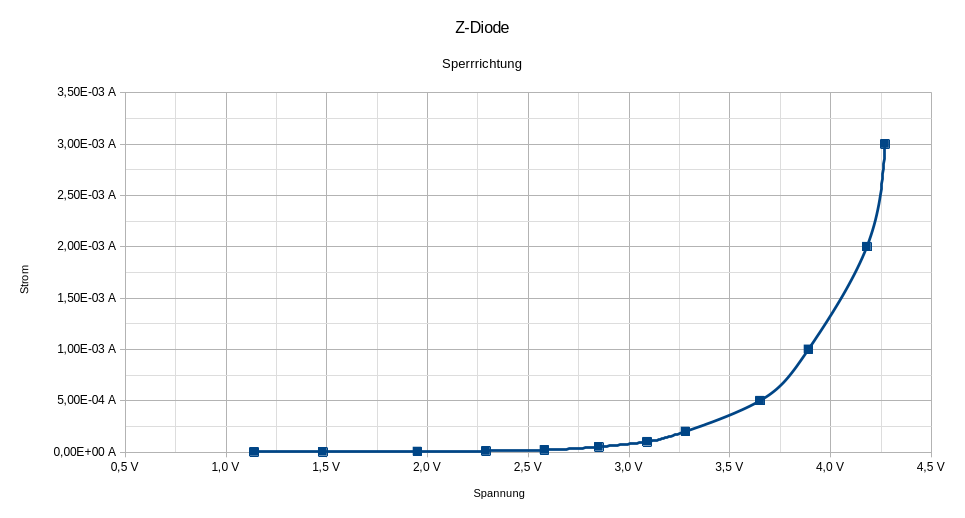
\includegraphics[width=0.85\textwidth]{img/4.1.a.6}
			      \caption{Z-Diode in Sperrrichtung}
		      \end{center}
	      \end{figure}

	      \pagebreak
	\item Berechnen Sie die Kennlinie der Si-Diode nach Gleichung 7, ermitteln Sie den Sperrstrom $I_s$ und den Emissionskoeffizienten m aus den Messungen. (Tipp: Den Emissionskoeffizienten bestimmen Sie, indem Sie zwei Messwerte in Gleichung 7 einsetzen und beide Gleichungen dividieren, so dass der Sperrstrom gekürzt werden kann. Diese Gleichung kann nun nach $m$ umgestellt werden.)
	\item Stellen Sie die gemessene und berechnete Kennlinie der Si-Diode im halblogarithmischen Maßstab dar (berechnete Kennlinie als Linie, Messwerte als Punkte).
	\item Beschriften Sie die fünf aufgenommenen Oszillogramme eindeutig.
\end{enumerate}

\pagebreak
\subsection{Temperaturabhängiger Widerstand}
\begin{enumerate}[label=\alph*)]
	\item Ermitteln Sie für jeden Messwert den Widerstand (Spannungsfehlerschaltung beachten!)
	      \begin{table}[h!]
		      \caption{Temperaturabhängiger Widerstand: Strom- und Widerstandswerte}
		      \begin{center}
			      \begin{tabular}[c]{c|c|c}
				      \hline
				      \multicolumn{1}{c|}{\textbf{Temperatur in $^\circ C$}} &
				      \multicolumn{1}{c|}{\textbf{Strom in $mA$}}            &
				      \multicolumn{1}{c}{\textbf{Widerstand in $\Omega$}}                     \\
				      \hline
				      22,5                                                   & 2    & 1000,00 \\
				      25                                                     & 2,2  & 909,09  \\
				      30                                                     & 2,4  & 833,33  \\
				      35                                                     & 2,7  & 740,74  \\
				      40                                                     & 2,9  & 689,66  \\
				      45                                                     & 3,5  & 571,43  \\
				      50                                                     & 4    & 500,00  \\
				      55                                                     & 5    & 400,00  \\
				      60                                                     & 6    & 333,33  \\
				      65                                                     & 6,7  & 298,51  \\
				      70                                                     & 8,6  & 232,56  \\
				      75                                                     & 10   & 200,00  \\
				      80                                                     & 10,5 & 190,48  \\
				      85                                                     & 13   & 153,85  \\
				      90                                                     & 15   & 133,33  \\
				      95                                                     & 20   & 100,00  \\
				      100                                                    & 35   & 57,14   \\
				      \hline
			      \end{tabular}
		      \end{center}
	      \end{table}
	      \begin{figure}[h!]
		      \begin{center}
			      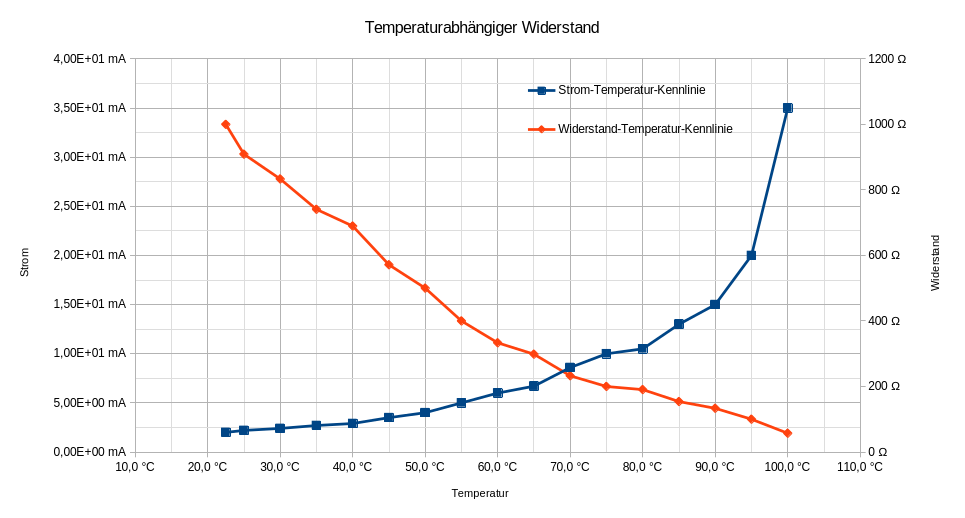
\includegraphics[width=0.95\textwidth]{img/4.2.a.1}
		      \end{center}
		      \caption{Strom-Temperatur-Kennlinie und Widerstand-Temperatur-Kennlinie}
	      \end{figure}
	      \pagebreak

	\item Berechnen Sie die Widerstandskennlinie näherungsweise nach Gleichung 8. Die Werkstoffkonstanten A und B sind aus den Messwerten bei minimaler und maximaler Temperatur zu ermitteln.
	      \begin{align*}
		      R(T)                                    & = A\cdot e^{\frac{B}{T}}                                                                \\
		      A                                       & = \frac{R(T)}{e^{\frac{B}{T}}}                                                          \\
		      \frac{R(T_1)}{R(T_2)}                   & = \frac{A}{A} \cdot \frac{e^{\frac{B}{T_1}}}{e^{\frac{B}{T_2}}}                         \\
		      \frac{R(T_1)}{R(T_2)}                   & = e^{\frac{B\cdot T_2-B\cdot T_1}{T_1\cdot T_2}}                                        \\
		      \ln \left(\frac{R(T_1)}{R(T_2)} \right) & = {\frac{B\cdot( T_2- T_1)}{T_1\cdot T_2}}                                              \\
		      B                                       & =\frac{\ln \left(\frac{R(T_1)}{R(T_2)} \right)\cdot {T_1\cdot T_2}}{( T_2- T_1)}        \\
		      B                                       & =\frac{\ln \left(\frac{1000\ \Omega}{57,14\ \Omega}\right)
		      \cdot {(295,65\ K \cdot 374,15\ K)}}{(374,15\ K - 295,65\ K)}                                                                     \\
		      B                                       & =4033\ K                                                                                \\
		      A                                       & = \frac{R(T_1)}{e^{\frac{B}{T_1}}} = \frac{1000\ \Omega}{e^{\frac{4033\ K}{295,65\ K}}} \\
		      A                                       & = 1,19\ m\Omega                                                                         \\
		      R(T)                                    & = 1,19\ m\Omega \cdot e^{\frac{4033\ K}{T}}                                             \\
	      \end{align*}
	\item Stellen Sie beide Kennlinien in einem Diagramm da (berechnete Kennlinie als Linie, Messwerte als Punkte).
    \begin{figure}[h!]
      \begin{center}
        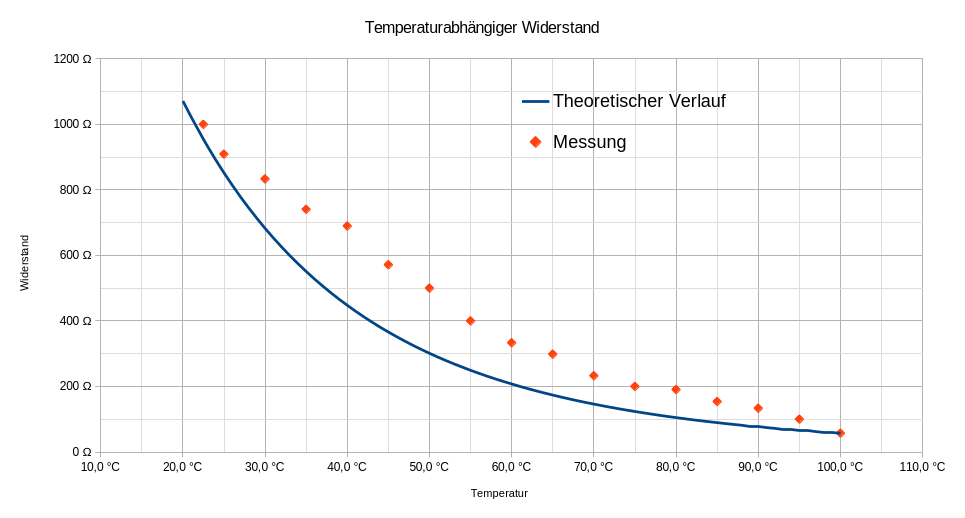
\includegraphics[width=0.7\textwidth]{img/4.2.c.1}
      \end{center}
      \caption{Widerstandskennlinie aus dem theoretischem Verlauf und der Messungen}\label{img:4.2.c.1}
    \end{figure}
    
    \pagebreak
	\item Vergleichen Sie die Kennlinien.
\end{enumerate}
\subsection{Transistor}
\begin{enumerate}[label=\alph*)]
	\item Stellen Sie die Eingangskennlinien nach 3.4.1 im linearen Maßstab in einem Diagramm dar.
    \begin{figure}[h!]
      \begin{center}
        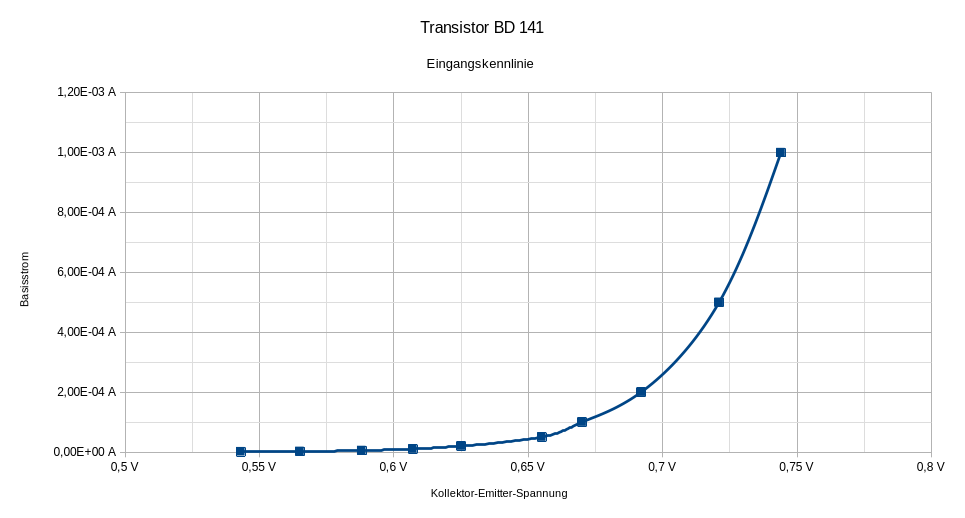
\includegraphics[width=0.85\textwidth]{img/4.3.a.1}
      \end{center}
      \caption{Eingangskennlinien des Transistors}
    \end{figure}
    
	\item Stellen Sie das Ausgangskennlinienfeld nach 3.4.2 im linearen Maßstab in einem Diagramm dar.
    \begin{figure}[h!]
      \begin{center}
        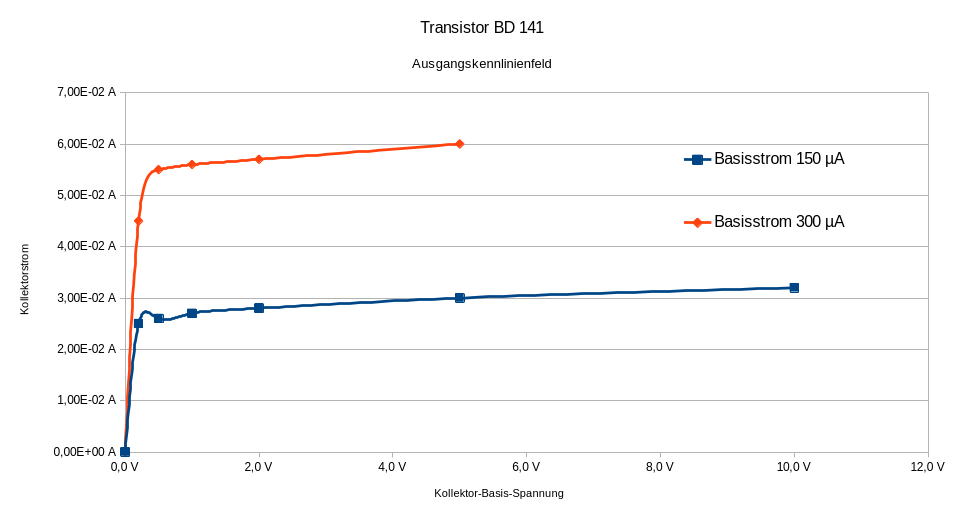
\includegraphics[width=0.85\textwidth]{img/4.3.b.1}
      \end{center}
      \caption{Ausgangskennlinienfeld des Transistors}
    \end{figure}

	\item Beschriften Sie das aufgenommene Oszillogramm eindeutig.
\end{enumerate}
